%*
%* Seven Kingdoms: Ancient Adversaries
%*
%* Copyright 1997,1998 Enlight Software Ltd.
%* Copyright 2018 Timothy Rink
%*
%* This program is free software: you can redistribute it and/or modify
%* it under the terms of the GNU General Public License as published by
%* the Free Software Foundation, either version 2 of the License, or
%* (at your option) any later version.
%*
%* This program is distributed in the hope that it will be useful,
%* but WITHOUT ANY WARRANTY; without even the implied warranty of
%* MERCHANTABILITY or FITNESS FOR A PARTICULAR PURPOSE.  See the
%* GNU General Public License for more details.
%*
%* You should have received a copy of the GNU General Public License
%* along with this program.  If not, see <http://www.gnu.org/licenses/>.
%*
%*

\chapter{Force and Its Use}

\section{The Fort}

\begin{wrapfigure}{l}{0.2\textwidth}
	\vspace{-20pt}
	\begin{center}
		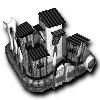
\includegraphics[width=0.2\textwidth]{Ifort}
		\\ Fort
	\end{center}
	\vspace{-20pt}
	\end{wrapfigure}

Your first Fort will be immediately visible when you begin a new game. \textbf{Click} on this Fort and you will see its only resident: your King. In order to issue commands to your Villagers, you must have a linked Fort staffed by either your King or a General. As your King has the highest level of leadership in your Empire and is already stationed there, there is no need to train any other leaders just yet. \\

\subsection{Conscription and Training}

In order to fill up your Fort and train Soldiers you must conscript Peasants into your armed forces.

\subsubsection{How do you conscript Peasants?}

\begin{wrapfigure}{r}{0.1\textwidth}
	\vspace{-20pt}
	\begin{center}
		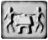
\includegraphics[width=0.1\textwidth]{Trecruit}
	\end{center}
	\vspace{-20pt}
\end{wrapfigure}

First \textbf{Click} on the Village whose Peasants you wish to conscript and then \textbf{Click} on the \textbf{Recruit Tile} once for each Peasant that you wish to conscript. You may recruit up to eight Peasants for each Fort.

After eight or fewer Peasants have been recruited and are standing outside your Village, \textbf{Group Select} them and then order them into the Fort with a \textbf{Right-Click} on the Fort.

An alternative method of conscription is to select the Village and then to \textbf{Right-Click} inside the rotating ring centered on the Linked Fort. For every \textbf{Right-Click}, one peasant will be transferred into the Fort to begin his training.

Soldiers who have been assigned to a Fort will no longer live in the Village. The Fort will become their new residence.

Because only Villagers pay taxes, having a large percentage of your subjects in the army will severely restrict your tax base.

\subsubsection{Combat and Leadership Levels}

Conscripted Soldiers will start off with a Combat Level and a Leadership Level of just 10. While they are training in their Fort or while they are fighting, their Combat Level will increase, the speed of increase depending on the Leadership Level of the General or King. If the commander’s Leadership Level is high, the soldier’s Combat Level will increase faster than if the commander’s Leadership Level is low.

The maximum combat level of any Soldier is 100.

A General’s or a new King’s Leadership will increase when training soldiers in a Fort or when men under his command and within 10 spaces of him are engaged in battle.

A soldier’s Combat Level will never increase beyond the Leadership Level of his commander.

Generals or Kings will gain an improve their Leadership Level only if they have soldiers and/or Weapons to command. The more units they have under their command, the faster their Leadership ability will increase.

In a small percentage of your common soldiers you may see a slow and steady increase in Leadership Level. These units should be watched and cultivated; they have an innate talent for Leadership, and may make excellent Generals one day.

Training units who have been wounded and then returned to the Fort will be slower than training units that are completely well. This applies to both Combat Level and Leadership Level.

An injured General will also improve his Leadership Level more slowly than an uninjured one.

On the field of battle, a General’s Leadership Level is of critical importance. A General or King imparts a combat bonus to members of his own Troop equal to his Leadership Level. For example, if a General has a Leadership Level of 100, a Soldier or Weapon in his Troop will receive a 100\% bonus to his combat ability. This assumes that the General (or King) is no more than 10 spaces away from each Soldier or Weapon. Keeping your Generals safely away from battle is therefore not a good idea.

Units who are not part of a General’s troop receive no combat bonus while fighting within 10 spaces of him.

\subsubsection{Hit-Point Bars}

Above the head of each selected unit, you will see a colored bar. There are three different colors that denote the maximum Hit-Points for any given unit.

A \textbf{Green} bar shows that the unit has a maximum of \textbf{between 20 and 50 Hit-Points}.

A \textbf{Yellow} bar shows that the unit has a maximum of \textbf{between 51 and 100 Hit-Points}.

A \textbf{Purple} bar shows that the unit has a maximum of \textbf{between 100 and the ultimate of 200 Hit-Points}.

\textbf{NOTE}: Although a unit may have only 5 Hit-Points remaining, only the length of the bar will change. The color will remain the same.

A unit’s possible Hit-Point plateau will be twice his present Combat Skill Level.

By paying attention to these colors it will be to see where your most valuable units are --- and those of your rivals.

All units will recover their Hit Points at the fastest rate when they are safe inside a building. They will also recover at a slower rate while they are outside but not moving. If they are on the move they will not recover.

\subsection{Unit Alertness Modes in Forts}

\index{alterness mode!in fort} You will have two options for the readiness of your troops inside their Fort: They may be ordered into either \textbf{Alert Mode} or \textbf{Stand Down Mode}.

\begin{wrapfigure}{r}{0.1\textwidth}
	\vspace{-20pt}
	\begin{center}
		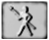
\includegraphics[width=0.1\textwidth]{Talert}
	\end{center}
	\vspace{-20pt}
\end{wrapfigure}

When in \textbf{Alert Mode}, your Troops and Weapons inside a Fort will immediately Sortie to fight any foe who is attacking either their Fort or anything Linked to it. If that foe is defeated, your troops will then return to their Fort.

In this situation your General will remain behind in the Fort directing operations. His leadership abilities will still influence his Troop and the Village to which the Fort is Linked.

\begin{wrapfigure}{r}{0.1\textwidth}
	\vspace{-20pt}
	\begin{center}
		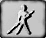
\includegraphics[width=0.1\textwidth]{Tstanddown}
	\end{center}
	\vspace{-20pt}
\end{wrapfigure}

When in \textbf{Stand Down Mode} your troops and weapons will stay safely behind the walls of your Fort until ordered otherwise. This may be a good idea if you are outnumbered and waiting for reinforcements.

\subsection{Unit Alertness Modes outside of Forts}

\index{alterness mode!outside fort} Outside of the Fort, troops in \textbf{Alert Mode} will behave with the intelligence that you would expect from real soldiers. They will automatically attack nearby enemy troops, (not civilians), but will not chase them out of the area unless so ordered by you. When attacking a structure they will break off to defend themselves against an enemy attack. If they defeat that attack, they will return their attention to the targeted structure.

If troops come under attack while they are on their way to an assigned destination, they will stop and fight the enemy. Then, if they are victorious, they will continue their journey.

Troops outside their Fort in \textbf{Stand Down Mode} will more blindly follow orders. When an enemy approaches, they will not attack unless they are attacked first. When marching to another location they will not stop to fight even when attacked, but will press on to their destination. They will only fight, in this case, if they are surrounded.

\clearpage

\subsection{Sortie}

\begin{wrapfigure}{r}{0.1\textwidth}
	\vspace{-20pt}
	\begin{center}
		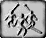
\includegraphics[width=0.1\textwidth]{Tsortie}
	\end{center}
	\vspace{-20pt}
\end{wrapfigure}

When your Fort is selected, \textbf{Click} the \textbf{Sortie Tile}. The entire strength of your Fort will then sally forth to do your bidding. They will exit the Fort as a single Troop, selected and ready to do battle.

To select the group again later, \textbf{Right-Click} on any of the Soldiers in the Troop. The entire Troop will then be selected and awaiting your orders.

When a Troop is selected you may order an attack on enemy Soldiers or on an enemy structure by \textbf{Right-Clicking} on the target. You will know that it is a valid target when your cursor turns red.

\subsection{Numbering Groups}

You may, if you wish, assign a number to a Troop, several Troops, or any group of people, Weapons, and / or Ships.

To do this, first \textbf{Select} or \textbf{Group-Select} the units that you want to number. Then press \textbf{Ctrl} + <\textbf{number 0–9}>.

To recall a numbered group, press \textbf{Alt} + <\textbf{number 0-9}>.

Troops in a numbered group will lose their number if they return to their Fort. You may not, therefore, recall a numbered troop from its Fort.

Remember that when a Troop is sortied from its Fort, it is already grouped as a single unit that can be easily selected by \textbf{Right-Clicking} on any of its members.

If you have numbered a group of two or more Troops you will still be able to select the individual Troops from within that group by \textbf{Right-Clicking} on any member. The selected Troop will still retain its assignment as a member of the numbered group if you wish to make use of it later.

\subsection{Selecting Units in a Crowd}

Selecting a single unit from within a crowd, or during a massive battle, can sometimes be difficult. To make it easier, hold down your \textbf{Ctrl key} while you \textbf{Click} on the area of the ground where the unit’s feet should be. The unit should then be selected. This selection method will work for all types of units.

\subsection{Withdrawal}

\begin{wrapfigure}{r}{0.1\textwidth}
	\vspace{-20pt}
	\begin{center}
		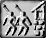
\includegraphics[width=0.1\textwidth]{Twithdrawl}
	\end{center}
	\vspace{-20pt}
\end{wrapfigure}

To return a selected Troop to their Fort, \textbf{Click} on the \textbf{Withdrawal Tile}. The Troop will immediately cease all present activity and march back to its Fort.

Even if your Troop is still being attacked, it will cease all fighting. In this case, the \textbf{Withdrawal Tile} will act as a quick retreat order. If members of a troop are surrounded by enemies and therefore cannot disengage from battle, they will continue fighting.

If you wish to send any selected units to another location, without them stopping for \textbf{\textit{any}} reason, \textbf{Double-Click} on their destination.

\subsection{Transfer}

To transfer a soldier or soldiers from one Troop to another, \textbf{Click} on or Group Select them and then send them into another Fort with a \textbf{Right-Click}. They will then become members of that Fort’s Troop.

\subsection{Waypoints}

To set waypoints for your People, Ships, or Weapons to follow, first select the unit(s). Then, holding down the \textbf{Alt} key, \textbf{Right-Click} on either the world map or your main screen. For each \textbf{Right-Click} you will set a waypoint. To set the last point, \textbf{Right-Click} without holding down the Alt key. Your selected units will begin to move as soon as the first waypoint has been set.

You may delete a waypoint (apart from the first) by \textbf{Right-Clicking} on the waypoint marker while the unit is selected.

Waypoints may \textbf{not} be used for Caravans or for Ships that are on trading routes.

\subsection{The Death of a King}

If your King has been slain in battle, you must immediately choose a successor to the Crown. The longer you wait, the more restless and rebellious your people will become.

\begin{wrapfigure}{r}{0.1\textwidth}
	\vspace{-20pt}
	\begin{center}
		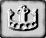
\includegraphics[width=0.1\textwidth]{Tcrown}
	\end{center}
	\vspace{-20pt}
\end{wrapfigure}

After the death of a King, upon selecting any unit, you will see the \textbf{Crown Tile} in the unit command bar. \textbf{Click} on this Tile if you want the selected unit to succeed to the Crown.

It is very important to your Empire that you select a unit with a high Leadership Level because if the new King’s Leadership Level is less than the old King’s, your people’s loyalty will drop.

Also bear in mind the nationality of the majority of your population. Selecting a King from within this national grouping may be the most prudent decision as the loyalty of people of Nationalities different from the new King will decrease.

Any other skills not befitting the station of a king, such as Spying, will be forgotten by a newly coronated unit. Combat and Leadership skills are retained.

\subsection{Restoring Unit Health}

All Soldiers who have been wounded will eventually regain their full strength if they are not moved. If they are returned to a Fort they will heal twice as fast.

\subsection{Weapons in Forts}

You may assign up to eight Weapons to a Fort, just as you would assign Soldiers. And just as with Soldiers, assigning a Weapon to a Fort commanded by a General makes the Weapon a part of that General’s Troop. When fighting within 10 spaces of the General, the Weapon and all other members of the Troop will receive a combat bonus equal to the General’s Leadership.

Your Weapons will be repaired in the Fort twice as fast as outside.

\subsection{Promotion, or How to make a General}

Each Fort, apart from the one that the King commands, needs a General to train the troops. A General is created by promoting a unit already trained in Leadership; that is, one who has been trained either directly from one of your Villages or one who has learned soldiering skills as a common Soldier in his Fort.

\subsubsection{How do you promote a Soldier?}

\begin{wrapfigure}{r}{0.1\textwidth}
	\vspace{-20pt}
	\begin{center}
		
\includegraphics[width=0.1\textwidth]{Tstar}
	\end{center}
	\vspace{-20pt}
\end{wrapfigure}

To promote a Soldier (with a small Sword Icon over his head) who is outside of a Fort, \textbf{Click} on him and then \textbf{Click} on the \textbf{Promote Tile}. His Sword Icon will change into a Star Icon, showing that he is now a General.

To promote a Soldier who is inside of a Fort that has no General in residence, first \textbf{Click} on the Fort. Then \textbf{Click} on the picture of the Soldier that you want to make into a General. The Soldiers are ranked from the top left in order of Leadership Level, so it is most likely that you will want to \textbf{Click} on the first Soldier. When his picture is highlighted in yellow, \textbf{Click} on the \textbf{Promote Tile}. That Soldier will become a General and take over command of the Fort. His picture will move to the General’s position on the top. You will also notice that his promotion increased his Loyalty Level by 20 points.

Your new general will now begin the training of those under him. At the same time his Leadership skills will steadily improve.

If a General has no one to train, his Leadership Skills will not increase.

\subsection{Demotion}

Assigning a new General to a Fort that already has a General will result in the old General standing outside. This General may be Demoted and reassigned to the Fort as a common Soldier or he may retain his rank and be assigned to build or command in another Fort.

\begin{wrapfigure}{r}{0.1\textwidth}
	\vspace{-20pt}
	\begin{center}
		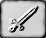
\includegraphics[width=0.1\textwidth]{Tsword}
	\end{center}
	\vspace{-20pt}
\end{wrapfigure}

To Demote, \textbf{Click} on the General and then \textbf{Click} on the \textbf{Demotion Tile}. This will return the General to the ranks of common soldiers.

When a General is demoted, his loyalty to you will decrease by 40.

Kings may not be Demoted.

\subsection{Honors}

\begin{wrapfigure}{r}{0.1\textwidth}
	\vspace{-20pt}
	\begin{center}
		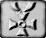
\includegraphics[width=0.1\textwidth]{Tmedal}
	\end{center}
	\vspace{-20pt}
\end{wrapfigure}

Honors are awards given to Soldiers (and other trained units) to help increase their level of loyalty. These Honors, although seldom deserved, cost money; but they can help ensure the happiness, loyalty, and obedience of your soldiers.

To Honor a Soldier or other unit, \textbf{Click} on him and then \textbf{Click} on the \textbf{Honors Tile}. Each time you do this, the unit’s loyalty will increase by 10 points and your treasure will decrease by \$30.

If you have a General who is making great Contributions to your cause, he will show his demand for increased Honors by a lowering of his Loyalty. Contribution is a tally of great deeds that a General has accomplished in his battles with enemy Kingdoms and with Fryhtans.

Generals also keep track of their Power. This is figured on the number of Soldiers under their command and their Combat Level. Also counted is the population of any Villages Linked to a Fort where a General is in command.

If a Village is Linked to more than one Fort, the Generals in charge of those Forts will perceive their Power to be lessened.

The more Contribution a General has made, the more power and Honors he will demand. If he is not given all that he feels he deserves, you will see a decrease in his loyalty.

\subsection{Betrayal}

\index{betrayal} If one of your Generals betrays you, some of the troops that he is commanding may join him and some may remain true to you.

If he is resident in a Fort he will capture the Fort. Those soldiers who do not wish to mutiny will exit and begin attacking the Fort.

If your turncoat General is in a Seat of Power he will capture it and all of the people inside.

When considering betrayal, a unit weighs the following factors:

\begin{adjustwidth}{1cm}{}
His own level of Loyalty

The Reputation of his Kingdom

The Power of his Kingdom

The Nationality, Reputation, and Power of the Kingdom that he is considering joining.
\end{adjustwidth}